\section{Density}
To measure the density in a uniform system consisting of just one atom type, we can use
\[
    \rho = \frac{Nm}{V},
\]
where $N$ is the number of atoms, $m$ the mass of an atom, and $V$ the volume of the whole system. But if we have a more complicated system, like in our case where we have three different atom types, liquid water in some parts of the system, and solid silica in other parts, we can not use that simple relation. What we do instead is to assiociate a volume $V_i^j$ with each atom of type $j$, and calculate the density of atom type $j$ using
\[
    \rho_j = \dfrac{m_jM}{\sum_{i=0}^M V_i^j},
\]
where $m_j$ is the mass an atom of type $j$, and $M$ is the number of atoms of type $j$. \hl{We identify as the $\rho_j/m_j$ number density.} We can find the mass of an atom type from standard tables of molar masses, but we still need to find the volumes $V_i^j$ associated with each atom. To do this we use something called \hl{Voronoi cells/Voronoi tesselation}\todobo{citation? Dirchlet 1850 and Voronoi 1908, so very old...}. Voronoi tesselation is done by dividing the system into non-overlapping convex polyhedra (or convex polygons in 2 dimensions), with one atom in each polyhedra. The volume inside the polyhedron surrounding each atom consists of all points in space closer to that atom than any other atom. 

We use the \cpp-library \texttt{Voro++} to find the Voronoi cells, and calculate the volumes of the cells. See \cref{fig:2d_voronoi_diagram} for an illustration of a 2-dimensional Voronoi, and \cref{fig:3d_voronoi_diagram} for a rendering of a 3D Voronoi diagram.
%
\begin{figure}[htpb]%
% \centering%
    \begin{minipage}[t]{0.485\textwidth}%
        \captionsetup{width=\textwidth}%
        \centering%
%         \includesvg[width=0.8\textwidth, svgpath=./images/voronoi/]{2d_diagram03}%
        \includesvg[height=0.7\textwidth, svgpath=./images/voronoi/]{2d_diagram06_overlapping}%
        \caption{%
            Illustration of Voronoi cells in 2 dimensions. Freely after Wikipedia Commons\cite{wikiVoronoiImage}.%
            \label{fig:2d_voronoi_diagram}%
        }%
    \end{minipage}%
    \hfill%
    \begin{minipage}[t]{0.485\textwidth}% % change "b" to "t" to anchor top instead of bottom
    \captionsetup{width=\textwidth}% % minipage defines a \textwidth for it's own, so we have to repeat this command inside the minipage
        \centering%
%         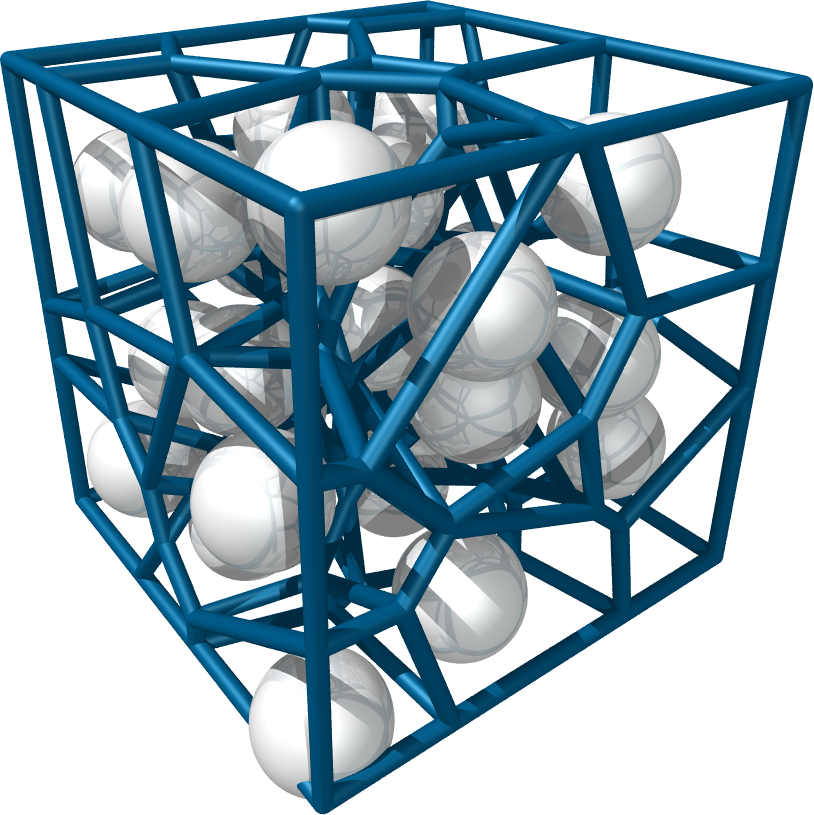
\includegraphics[width=0.8\textwidth]{images/voronoi/3d_diagram04_crop.png}%
        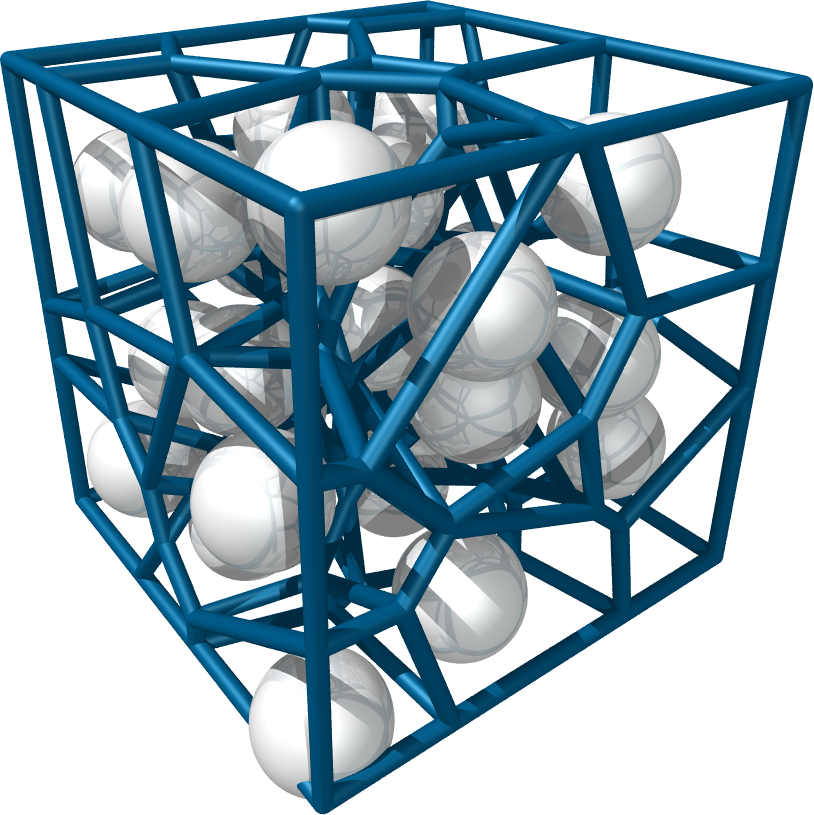
\includegraphics[height=0.7\textwidth]{images/voronoi/3d_diagram04_crop.png}%
        \caption{%
            Rendering of Voronoi cells in 3 dimensions, in a system of 27 particles. Voronoi cells created using the \cpp-library \texttt{Voro++}\cite{rycroft2009voro,webvoro++}, and rendered using the program \texttt{povray}\cite{webpovray}. %
            \label{fig:3d_voronoi_diagram}%
        }%
    \end{minipage}%
\end{figure}%

\todoa{Something about removing hydrogen atoms, and just use oxygen position as hydrogen position, and water atom ``volume''? This simplifies life for us, since we do not have to find which water molecule each hydrogen atom belongs to, but we could get inconsistent water density. But since we use the same method for all measurements, we can compare relative densities.}

\todoa{Write about averaging over timesteps and atoms}

\todob{Something about removing extreme points/tail in distribution? Caused by vacuum.}